
\chapter{Process}
\label{processSec}
This project is largest project the author has solely been responsible for however, this does not define the project as a large project. The author is working alone and does not have a dedicated team as assistance. This combined with the fact that the time frame which the project has to be completed in has lead the author to come to the conclusion that there is no single Process Model that would be entirely suited for him and this project. The lack of one specific process gives the author the temptation to fall back on process at all however, the lack of any rational structure is vastly inappropriate for this project.
Rather than using one single process, the author feels that is can modify existing processes in order to create a process which captures the necessary principles required in order to create a logical structure which can be applied effectively to this project. Agile methodologies are often used in small development teams, specifically eXtreme Programming (XP). XP places heavy importance of quality and responding to customer demands through the use of multiple iterations and a simple design process (compared to planned design). However, small development teams are using XP as a scapegoat for not adhering to a specific process or methodology. XP is still very much focused around a team of people working are there is constant deliberation about XP and its adaptation to single developer project such as this \cite{XP:forone}. However, there are XP principles which are well suited to this style of project for example, there is less emphasis on a heavy design process allowing for a more flexible development process which has been vital for this project in particular as the proposed design had to be significantly changed during development (more details can be found in section \ref{DesignSec}). The author feels that in a solo project, the ability to be flexible and independent of any concrete design is key to a successful project. As the author has created a brief design specification individually without the help of a specialised team (see appendix B) there is the possibility that there are some key elements missing which may not be noticed until the implementation stage. XP flexibility effective makes this a non-issue during development as it accounts for the projects features to change, if the author adopted a strict plan based methodology then this maybe an issue.

As stated the process used is a hybrid process containing relevant ideologies from other software development processes. In conjunction with XP principles discussed above, the author has decided that there has to be some planned process involved in the projects development. The idea behind using a planned approach as the main underlying process is because the author feels that when working on solo projects it is easy to get lost in terms of what goals still need to be achieved. This planned process won’t be as strict as it would be if a planned approach was the sole process being used for this project, instead the design and requirements processes will be much shorter than usual and will only cover the main requirements and overall system interactions. 

\begin{figure}[h!]
\centering
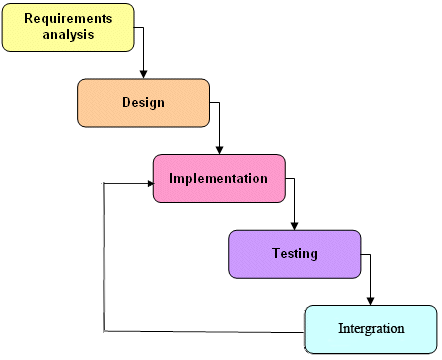
\includegraphics[scale=0.7]{Images/chapter3/waterfallmodel}
\caption{The varation of the waterfall model used for solo development in this project. Modified from source image \cite{waterfall:image} }
\label{fig:waterfall}
\end{figure}

Figure \ref{fig:waterfall} represents the variation of the waterfall model used as part of the hybrid process in this project. The general waterfall structure has remained the same, the process starts off with a problem analysis stage which is reflected in appendix A and chapter \ref{chap:analysis}. With the introduction of the XP principles, the design stage is reduce in its complexity. This is with the intent to reduce how concrete the design is and also reduce the amount of time spent on the formal design of the application. The main adaptation comes from the approach to implementation and testing. As in introduction of XP has enabled the author to be more flexible in the implementation process if a new feature or refactoring is required, rather than going back to the design stage, this new process allows the author to implement the change or refactored code, test the changes and integrate the changes into the current working application. This saved tremendous amounts of time during the development process. Each change is handled in small sections rather than implementing several changes at once, each change will be broken down into logical section which will each in turn go through the implementation and testing process. This process continues until the requirements define in appendix A have been adhered to. This hybrid process is based on the work by Tom Blanchard \cite{tblanch:diss}, the process is very effective for use in solo projects.